\label{Design}
\subsection{Physical Environment}
\label{Design:PhysicalEnvironment}
The real-world environment in which the user will be tracked is approximately 12ft x 22ft.
The user is provided with a Head-Mounted Display and two 6 Degree of Freedom (6DOF) devices with 11 buttons each (Wiimotes) (see Figure \ref{fig:wiimote}).
The tracking of the head and each Wiimote is done with a Vicon system placed around the tracking area.

\begin{figure}[htbp]
	\centering
	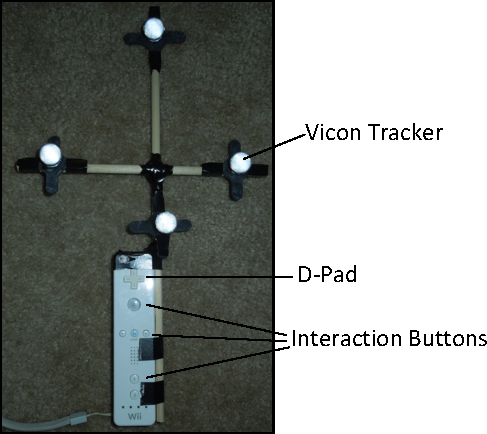
\includegraphics[width=3in]{figs/wiimote.pdf}
	\caption{Wiimote with Vicon trackers}
	\label{fig:wiimote}
\end{figure}

\subsection{Virtual Environment}
\label{Design:VirtualEnvironment}
The virtual environment is an empty and infinite 3D canvas for the user to create a virtual world.
This allows the user to create any object, building, landscape, or geometrical feature that is possible, with any size imaginable.
Since the user is creating a world, there are no sounds, animations, or simulation effects in place to begin with.
However, the user may create any item within the world, which can be utilized to create moving objects, 3D sounds, and simulation effects.
For instance, the user can create a car that moves along a street, with associated engine and tire noise as it moves.
The user could also create the ground and say that objects must ``rest'' upon the ground (simulating gravity).

\subsection{Interaction}
\label{Design:Interaction}

\subsubsection{Selection}
\label{Design:Interaction:Selection}
Object selection is a crucial task for most of the features within this project.
We will be augmenting object selection with tactile feedback provided through the Wiimote's rumble feature.
When a user selects a new object, the Wiimote will rumble for a predetermined amount of time.
Several selection selection methods are provided, which can be selected based on the users preference.
\begin{itemize}
	\item Virtual Hand Casting
	\item PORT
\end{itemize}

\paragraph{Virtual Hand Casting}
Virtual Hand Casting is a novel hybrid technique combining Virtual Hand and Ray Casting.
A virtual hand will be co-located with the user's real hand.
In additon, a ray is shot from the user's hand to enable object selection at a distance.
Once an object is selected, manipulation of an object follows a 1:1 mapping of the movement of the user's hand similar to the Virtual Hand technique.
This enable high fidelity manipulation of objects regardless of distance.
In addition to the hand co-located with the user's hand, a ``laser pointer'' can be enabled which follows the ray.
This enables higher fidelity of object selection.
Lastly, we draw a bounding sphere around the object(s) which the user is pointing at as well as the currently selected object(s).

\paragraph{PORT}
The user can create a 3D selection box where all objects within the box become selected.
This selection method provides the most flexibility, especially within our application, however the cognitive overhead on the user is  higher.
Once a user is proficient with the system, we believe this will be a frequently used selection method.

\subsubsection{Manipulation}
\label{Design:Interaction:Manipulation}
There are several manipulation techniques provided.
\begin{itemize}
	\item Single-Object Manipulation
		\subitem Creation
		\subitem Deletion
		\subitem Translation
		\subitem Rotation
		\subitem Scaling
		\subitem Coloring
		\subitem Texturing
	\item Multi-Object Manipulation
		\subitem Boolean Operations
		\subitem Grouping
		\subitem Deletion
	\item World Manipulation
		\subitem Scale-the-World
		\subitem Light creation/manipulation
		\subitem Sound creation/manipulation
\end{itemize}

\paragraph{Single-Object Manipulation}
This subcategory of manipulation is dedicated to a user manipulating one object at a time.
Creation and deletion will be done through a menu (described \ref{Design:Interaction:SystemControl}), however deletion will require an object to be selected first.
Translation, rotation, and scaling will all be performed with button interaction on the Wiimote, after an object is selected.
Scaling is unique, as it requires bimanual input.
The user must select and object, press buttons on both Wiimotes, and move both hands for the object to be scaled.
The actual motion will be determined by the hand movement while the interaction button is being held down.
Coloring and texturing will also be performed through a menu (see \ref{Design:Interaction:SystemControl}) and will also require an object to be selected first.

\paragraph{Multi-Object Manipulation}
There are three boolean operations using multiple objects provided.  Boolean operations can be performed when there are overlapping portions of multiple selected objects.
\begin{enumerate}
	\item Union
	\subitem When the user selects the union operation and multiple objects are selected, it creates a single, fused, object made up of all the objects that were selected.
	\item Intersection
	\subitem When intersection is selected, the non-overlapping portions of the selected objects will be removed, leaving a single object made up of only the intersecting portion.
	\item Subtraction
	\subitem This operation is limited to two selected objects.  When subtraction is selected, the user chooses a primary object, and the overlapping portion of the primary object is removed.  This operation leaves two objects, however the primary object is now missing the overlapped portion.
\end{enumerate}

Grouping objects allows the user create a single object from a group of selected objects.
Unlike the boolean operations, no logic is performed on the group other than making them behave as a single object.
The grouped objects, for all intents and purposes, behave as a single object, all the single object manipulations above work on a grouped objects.
One benefit grouped objects provide over the boolean operations, is that it can be undone.
Multiple objects can be grouped, manipulated, ungrouped, and manipulated independently.
Grouping objects will be performed through the menu described in \ref{Design:Interaction:SystemControl}.

Deletion is the same as single-object deletion, however it allows the user to delete multiple, unconnected objects (as long as all are selected).

\paragraph{World Manipulation}
When the user grabs the air with both hands, and performs the scaling operation, the entire world will be scaled up or down, according to the user's movement.
This allows the user to navigate more easily, as well as create very large structures within the virtual environment without too much effort (simply scale the world down, create a normal object, and scale the world back to normal size).

Light creation and manipulation allows the user to create lights, move them, and change aspects of the lights to suit the application (color, attenuation, direction, etc...).\footnote{Technical note: We are using OpenGL, so the number of lights in the world is limited to 8.}
The same ability exists for sounds.
The user can create a sound, attach it to an object, and the sound is then created from a specific point in space.

\subsubsection{Navigation}
\label{Design:Interaction:Navigation}
Navigation is another crucial feature.
Since the world is infinite, there must be a sensible way to navigate, otherwise the world will be limited to the size of the tracked area.

The main method of navigation will be real walking, since we have a 12ft x 22ft space, the user will be able to walk in any direction within the space, and that motion will be translated to the virtual environment.
Another navigation mechanism provided will be virtual walking.
We will be using the D-Pad on the Wiimote to simulate a joystick.
i.e. If the user presses ``Up'' on the D-Pad, they will move forward in the virtual environment.

Another navigation feature is to use the manipulation feature Scale-the-World.
Since the user can scale the entire world down, they can make everything smaller, making their steps (both real and virtual) much larger.
This method loses some interaction fidelity for the benefit of an infinite world.

\subsubsection{System Control}
\label{Design:Interaction:SystemControl}
As mentioned before, a menu will be present.
The menu is created in 3D space where the user's right hand is when activating the menu.
The menu is a collection of categories laid out in tabs, with buttons under each tab for the functions available in that category.
The categories provided are:
\begin{itemize}
	\item Objects
	\subitem Allows the creation of default objects (sphere, cube, cone, etc...)
	\item Materials
	\subitem Contains a collection of colors and textures to apply to objects
	\item Tools
	\subitem All of the advanced interaction methods listed above
	\item File Operations
	\subitem This category is unique, as it doesn't pertain to editing the world.  This category contains operations to save the existing world to file, load a file as an existing world, export an object to use again later, and load an object that was previously exported.
\end{itemize}


See Figure \ref{fig:menu} for a mock-up of the menu.

\begin{figure}[hp]
	\centering
	\subfigure[Object Menu] {
		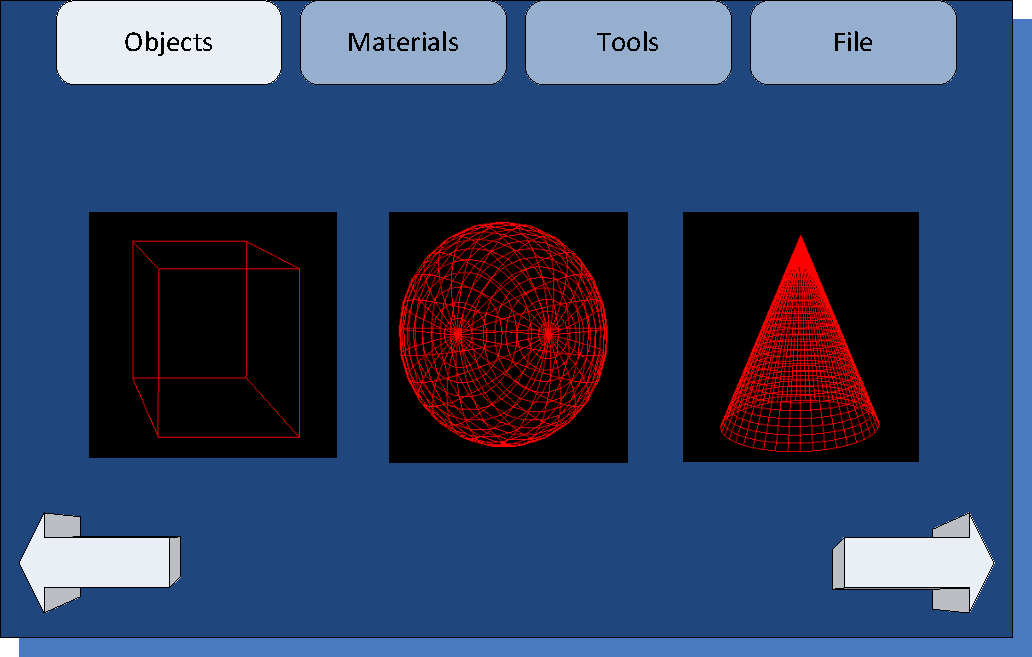
\includegraphics[width=3in]{figs/object_menu.pdf}
	}
	\subfigure[Material Menu] {
		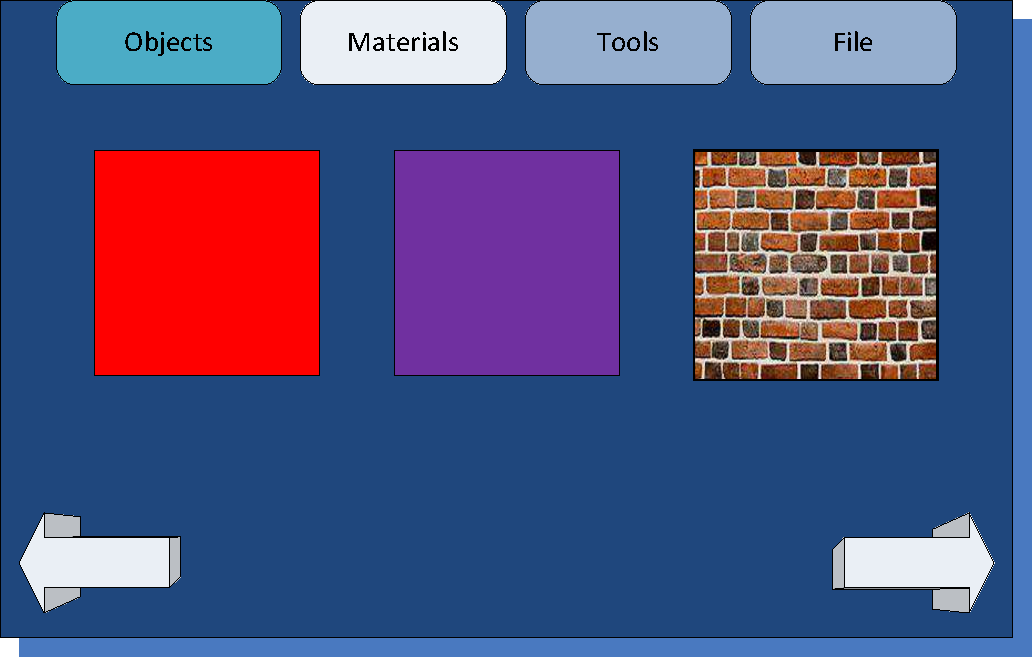
\includegraphics[width=3in]{figs/material_menu.pdf}
	}
	\subfigure[Tools Menu] {
		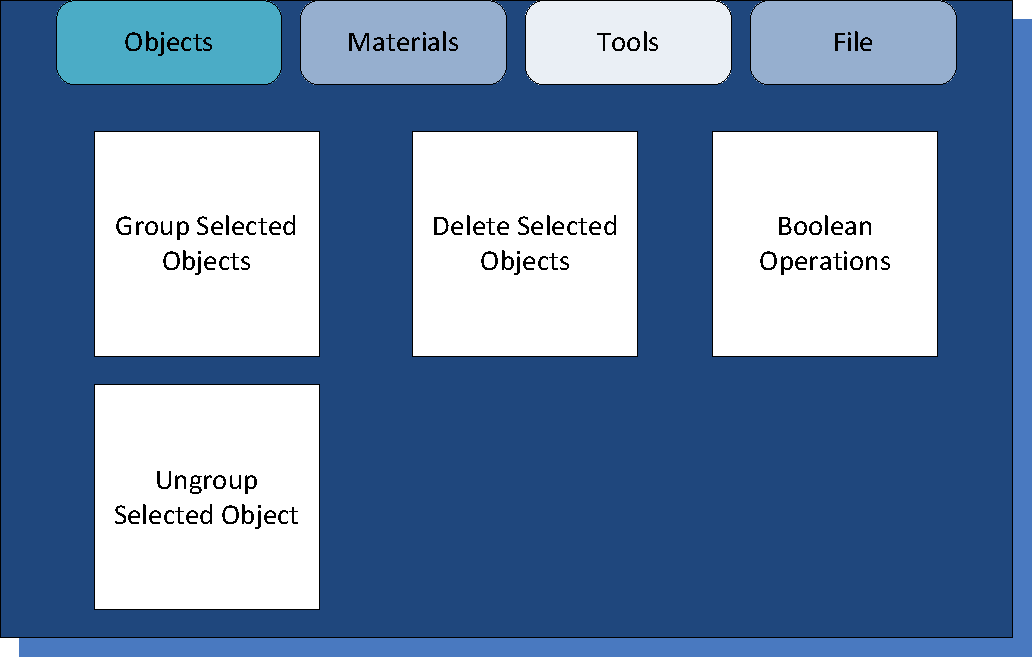
\includegraphics[width=3in]{figs/tools_menu.pdf}
	}
	\subfigure[File Menu] {
		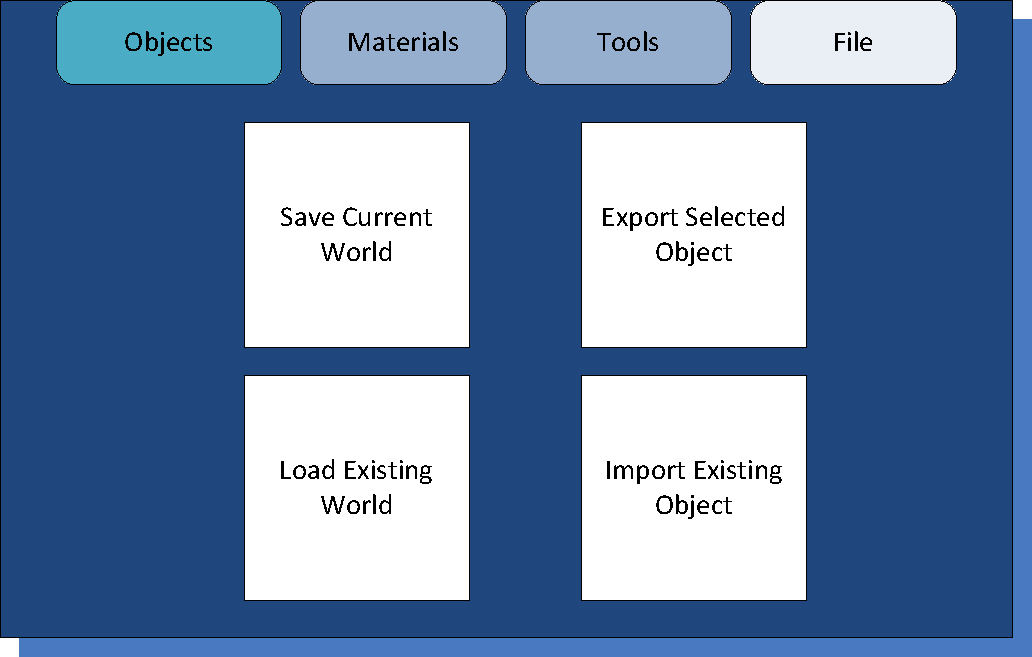
\includegraphics[width=3in]{figs/file_menu.pdf}
	}
	\caption{Mock up menu interface}
	\label{fig:menu}
\end{figure}

\subsubsection{Grammar based Production of Objects}
\label{Design:Interaction:GrammarBasedProduction}
A grammar or rule based production of objects will allow to specify a set of rules to the application, either pre-set or user programmable
that will automatically create objects in the pattern specified by the rule. This feature may be implemented in two ways. One in which the user 
directly specifies the production rules or recipe to create the object in the specified pattern and second, the system learns the underlying 
grammar or pattern from a set of exemplars created or loaded by the user. However this is an advanced feature and maybe beyond the scope of the
current project.

